% Created 2016-09-08 Do 16:45
\documentclass[a4paper,12pt,oneside]{book}
\usepackage[DIV=12,BCOR=2mm,headinclude=true,footinclude=false]{typearea}
\usepackage[utf8]{inputenc}
%\usepackage[T1]{fontenc}
\usepackage[german]{babel} 
%\usepackage{kpfonts}
%\usepackage{mathptmx}
%\usepackage{times,mtpro2}
\usepackage{stix}

\usepackage{url}
\usepackage{tabularx}

%\usepackage{txfonts}
%\usepackage{newtxtext,newtxmath}
%\usepackage{libertine} \usepackage[libertine]{newtxmath}
\usepackage{listings}
\usepackage{color}
\usepackage{textcomp}
\definecolor{bluekeywords}{rgb}{0,0,1}
\definecolor{greencomments}{rgb}{0,0.5,0}
\definecolor{redstrings}{rgb}{0.64,0.08,0.08}
\definecolor{xmlcomments}{rgb}{0.5,0.5,0.5}
\definecolor{types}{rgb}{0.17,0.57,0.68}

\usepackage{listings}
\lstset{language=[Sharp]C,
	captionpos=a,
	basicstyle=\fontfamily{consolas}\selectfont
	framextopmargin=26pt,
	framexbottommargin=26pt, 
	frame=tb, framerule=0pt,
	showspaces=false,
	showtabs=false,
	breaklines=true,
	showstringspaces=false,
	breakatwhitespace=true,
	escapeinside={(*@}{@*)},
	commentstyle=\color{greencomments},
	morekeywords={partial, var, value, get, set},
	keywordstyle=\color{bluekeywords},
	stringstyle=\color{redstrings},
	basicstyle=\ttfamily\small,
}


\usepackage{fixltx2e}
\usepackage{graphicx}
\usepackage{grffile}
\usepackage{longtable}
\usepackage{wrapfig}
\usepackage{rotating}
%\usepackage{cite}
\usepackage{cite}
\usepackage[normalem]{ulem}
\usepackage{amsmath}
\usepackage{textcomp}
\usepackage{amssymb}
\usepackage{capt-of}
\usepackage{hyperref}
\author{Dennis Müller}
\date{\today}
\title{}
\hypersetup{
 pdfauthor={Dennis Müller},
 pdftitle={},
 pdfkeywords={},
 pdfsubject={},
 pdfcreator={Emacs 24.5.1 (Org mode 8.3.6)}, 
 pdflang={English}}
\begin{document}


\chapter{Vision}
\label{sec:orgheadline8}
Im Grunde geht es bei einem Editor für Flow Design vorallem darum die Vorteile aus der digitalen Welt mit
der Methodik zu vereinen, ohne die Einfachheit der Methodik auf dem Papier zu
verlieren. 

\section{Vorteile eines digitalen Editors}
\label{sec:orgheadline6}
Flow Design ist eigentlich als Entwurfsmethode auf dem Papier gedacht.
Jedoch hat ein Flow Design auf dem Papier einige Nachteile, die ein Editor am
Computer aufheben könnte. Das wären vorallem folgende Punkte:
\subsubsection{Einmal eingezeichnete Pfeile, Kreise und Beschriftungen lassen sich nicht so leicht mehr verändern.}
\label{sec:orgheadline1}
Während des kreativen Prozesses ein Programmierproblem zu lösen, bedarf es
mehrer Iterationen und Veränderungen an dem Diagramm. Eine Möglichkeit Versionen
abzuspeichern und Teile zu verschieben, umzubenennen und umzustukturieren sind
klare Vorteile von einem digitalen Editor.
\subsubsection{Automaische Validierungsprozesse}
\label{sec:orgheadline2}
Während der Erstellung des Flow Designs können im Hintergrund
Validierungsprozesse beim Erstellen des Diagrammes Hilfestellung bieten.
Autovervollständigungen könnten ebenfalls an einigen Stellen eingebaut werden,
um das Tippen zu beschleunigen.
\subsubsection{Unnötige Abtipparbeit ersparen.}
\label{sec:orgheadline3}
Aus den Beschriftungen im Flow Design Diagramm lassen sich die Variablennamen und
Methoden Signaturen leicht herleiten. Liegt das Diagramm in digitaler Form vor,
wäre eine automatische Generierung von Quellcode naheliegend und
würde dem Anwender unnötige Abtipparbeit ersparen.
\subsubsection{Generierung von Methoden-Bodies}
\label{sec:orgheadline4}
Durch die strikten Implementierungsregeln von Integrationen lassen sich von
diesen Methoden nicht nur die Signaturen, sonder sogar die komplette Implementierung aus dem Diagramm
ableiten. Eine Generierung dieser Codezeilen wäre ein zustätzlicher Komfortgewinn von einem Editor.
\subsubsection{Roundtrip-Engineering}
\label{sec:orgheadline5}
Eine Möglichkeit aus einer bestehenden Codebasis ein Diagramm zu erstellen -
wenn auch nur teilweise - würden die Produktivität beim Einsetzen von Flow
Design in einem Projekt weiter steigern. Aufgrund von Unterhaltungen mit meinem
Anleiter Kevin Erath stellte sich heraus, dass ein perfekter Roundtrip umzusetzen keine triviale Aufgabe
darstellt. Deswegen wird im Rahmen dieser Arbeit der Fokus auf jene Funktionalitäten
gelegt, die leichter zu implementieren sind und doch dem Anwender möglichst viel
Zeitersparniss einbringt. Ein Anwendungsfall wäre: Der Anwender möchte
Teile seines Quellcodes in ein Flow Design überführen, um dann mit Hilfe des
Flow Designs, diesen zu überarbeiten und anschließend neu zu generieren.
Möglicherweise würde er die erstellten Codezeilen mit Copy-Paste in sein
bestehendes Projekt übertragen.

\section{Vorteile von einem Entwurf auf dem Papier}
\label{sec:orgheadline7}
Ein Papier schränkt einen nicht ein und erlaubt es schnell und einfach Pfeile
und Kreise zu zeichnen, Notizen einzufügen und ist einfach in der Bedienung.
Bei dem Erstellen eine Editors muss deshalb ein besonders großes Augenmerk auf
eine gute und intuitive Bedienung gelegt werden, damit einem das Programm bei der kreativen Arbeit nicht
behindert. Endziel wäre es, dass der Andwender von sich aus lieber zum Edtior
greift, als zu Stift und Papier, weil ihm der Editor komfortableres und
kreatives Arbeiten besser ermöglicht.

\chapter{Anforderungen}
\label{sec:orgheadline21}
\section{Editor}

\begin{tabularx}{\textwidth}{X|l}
Anforderungen & Priorität\\
\hline
Erstellen von Softwarezellen, Benennen, Verschieben auf dem Canvas, Löschen, Duplizieren & hoch\\ \hline
Navigation ( Panning, Zooming ) & hoch\\ \hline
Selektieren von mehreren Softwarezellen um mehrere auf einmal zu bearbeiten & hoch\\ \hline
Definieren von Input und Output Datastreams, für eine Softwarezelle & hoch\\ \hline
Verbinden eines Outputs einer Softwarezelle mit einem Input einer anderen & hoch\\ \hline
Zusammenlaufen von mehreren Datenflüssen in ein Input einer Softwarezelle & hoch\\ \hline
Softwarezelle(n) einer anderen unterordnen können, um Integrationen zu erstellen inklusive visuelle Kennzeichnung & hoch\\ \hline
Speichern und Laden in ein Dateiformat & hoch\\ \hline
Softwarezellen Klassen zuordnen & mittel\\ \hline
Syntaxhighlighting für die Datentypen auf den Datenflüsen & mittel\\ \hline
Keyboard Hotkeys / Tabstops & mittel\\ \hline
Automatisches Spacing & mittel\\ \hline
Validierung von Datenströmen & mittel\\ \hline
Untergeordenete Softwarezellen einer Integration an einer anderen Stelle definierbar machen, falls Platz knapp wird & mittel\\ \hline
Autosave & mittel\\ \hline
Undo / Redo System & mittel\\ \hline
Definieren von State einer Softwarezelle & mittel\\ \hline
Definieren von neuen Datentypen & mittel\\ \hline
Mouse-Hover zeigt Preview des erzeugten Codes für die Softwarezelle & niedrig\\ \hline
Wiederverwenden von vorhandenen Softwarezellen & niedrig\\ \hline
Autocomplete auf dem Textfeld der Datenströme & niedrig\\ \hline
Kommentarboxen & niedrig\\ \hline
Anfügen von Tests an Softwarezelle & niedrig\\ \hline
Mehrere Themes: Dark, White (Print) & niedrig\\ \hline
\end{tabularx}

\subsubsection{Anmerkungen}
\label{sec:orgheadline10}
\begin{enumerate}
\item Navigation
\label{sec:orgheadline9}

In Anlehnung an der Bedienung einger Grafikprogrammen:
Panning ( Verschieben der "Kamera" in
der X- und Y-Achse mit Hilfe der Mittleren Maustaste. Zoomen in und aus dem
Diagramm durch das Mausrad. Die Position der Maus bestimmt das Zentrum des
Zooms.
\end{enumerate}




\section{Generierung von Code}
\label{sec:orgheadline16}

\begin{tabularx}{\textwidth}{X|l}
Anforderungen & Priorität\\
\hline
Generierung von Methodensignaturen aus dem Namen und Input/Output Definitionen einer Softwarezelle & hoch\\
\hline
Erzeugen des kompletten Methoden-Bodies einer Integration & hoch\\
\hline
Erzeugung von Klassen und Datentypen & hoch\\
\hline
Einstellungen  dem Benutzer zugänglich machen, um die Generierung zu konfigurieren & mittel\\
\hline
Erzeugung von Namenspaces und Ausflösung von Usings & niedrig\\
\hline
Korrektes Einfügen / Integrieren von den generierten Codezeilen in die Codebasis eines bestehendes Softwareprojektes & niedrig\\
\hline
Live-Generierung & niedrig\\
\hline
\end{tabularx}


\subsubsection{Anmerkungen}
\label{sec:orgheadline15}
\begin{enumerate}
\item Erzeugung des kompletten Methoden-Bodies einer Integration

Hierbei muss erkannt werden, in welcher Reihenfolge die Methoden aufgerufen
werden müssen, lokale Variablen erzeugt werden müssen und was einer Methode als Parameter
übergeben werden muss. Dabei kommen IEnumerables und Lampdas zum Einsatz um
Datenflüsse zu implementieren. 

\item Einstellungen für die Generierung dem Benutzer zugänglich machen
\label{sec:orgheadline13}

Mögliche Optionen wären:

- wie das Programm den Methoden-Body einer Operation standardmässig befüllen soll: Leer, mit NotImplementedExeption oder mit einem
Default return Ausdruck abhängig von der Methodensignatur. 

-Ob innerhalb einer Integration der Rückgabewert einer Funktion erst in eine
lokale Variable gespeichert werden soll, oder direkt der Methodenaufruf an die
andere Methode weitergereicht wird. Beziehungsweise die Regel konfigurierbar
machen: Ab welcher Zeilenlänge, wie die Varibalen benannt werden sollen, etc.


\item Einfügen von generierten Codezeilen in bestehende Codebasis
\label{sec:orgheadline14}

Notwendig hierfür wäre, dass bestehende Klassen gefunden werden müssten, usings korrekt
eingefügt und schlussendlich die generierten Methoden und Datentypen in die
jeweiligen Klassen / Dateien eingefügt werden. Dabei muss die Syntax
berücksichtigt werden und möglicherweise Zugriffsberechtigungen erkannt und bei
Problemen einen Dialog zur Korrektur dem Anwender anbieten. Weiteres Problem
wäre die Überschneidung von Namen. 

Wenn automatisch der generierte Code bevorzugt
  werden soll, dann könnten durch die Überschreibung von Datentypen und Methoden
  bestehende Codezeilen plötzlich fehlerhaft werden. Ein extra Dialog wäre
  möglich, würde jedoch den Aufwand zur Integration des Codes möglichweise stark
  anheben. Ebenso wäre ein solcher Dialog aufwendig zu implementieren.
 
  Eine andere Option wäre es, dies Codezeilen einfach einzufügen und die Erkennung und Lösung der
  Probleme der IDE zu überlassen. Gerade bei C\# gibt es mit Resharper viele
  Refactorisierungs-Tools, die einem bei der Lösung solcher Probleme unterstützen.
\end{enumerate}


\section{Generierung von Flow Design Diagrammen aus Code}
\label{sec:orgheadline20}

\begin{tabularx}{\textwidth}{X|l}
Anforderungen & Priorität\\
\hline
Finden von Methoden und Erzeugen von Softwarezellen und ihre Input und Output Datenströme anhand der Methodensignatur im Code & hoch\\ \hline
Automatisches Spacing & hoch ( aber nicht unbedingt perfekt)\\ \hline
Den Datenfluss einer Integration erkennen und ihn in ein Flow Design Diagramm übertragen & hoch\\ \hline
Erkennen, ob es sich bei der Methode um eine Operation oder Integration handelt & hoch\\ \hline
Umgang mit Methoden die nicht das IOSP befolgen & mittel\\ \hline
Speichern der Inhalte, die nicht im Diagramm dargestellt werden können. & mittel\\ \hline
\end{tabularx}

\subsubsection{Anmerkungen}
\label{sec:orgheadline19}
\begin{enumerate}
\item Automatische Anordnung
\label{sec:orgheadline17}

Unbedingt notwendig, auch wenn es nur sehr rudimentär umgestetzt wird, ansonsten liegen
alle Softwarezellen nach dem Erstellen unübersichtlich auf einem Punkt aufeinander.
Falls das Automatische Spacing an manchen Stellen nicht perfekt funktionieren
sollte, kann eine gute Usability ( Selektierungs- und Verschiebungsfeatures)
hier dieser Imperfektion leichter verschmerzbarer machen.

\item Schwierigkeiten
\label{sec:orgheadline18}

Bei Verwendung von Events kann der Datenfluss möglicherweise nicht mehr
nachvollzogen werden.
\end{enumerate}

\pagebreak
\chapter{GUI Skizzen / Usabilityüberlegungen}
\label{sec:orgheadline28}

\section{Minimalistischer Aufbau. Fokus auf Produktivtät.}
\label{sec:orgheadline22}

Die Hauptansicht

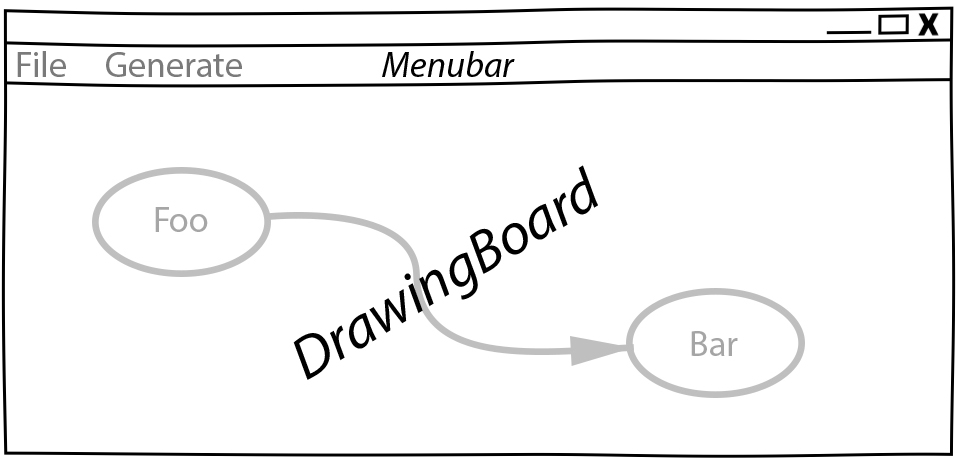
\includegraphics[width=.9\linewidth]{./img/MainCrop.jpg}

Die Anwendung soll möglichst viel Platz für die Zeichenfläche
bieten.

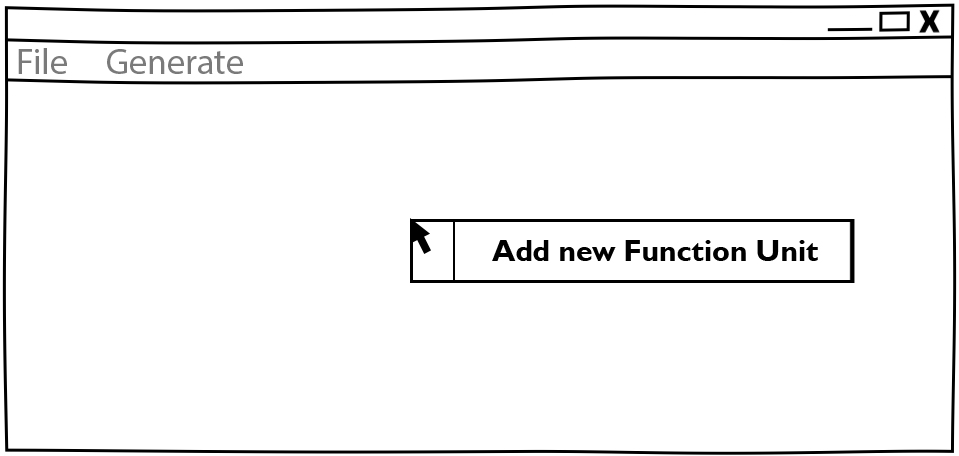
\includegraphics[width=.9\linewidth]{./img/ContextMenu.jpg}

Bei einem Rechtsklick auf eine leere Stelle in der Zeichenfläche erscheint ein
Kontextmenu, dass dem Anwender erlaubt an dieser Stelle eine neue Softwarezelle einzufügen.

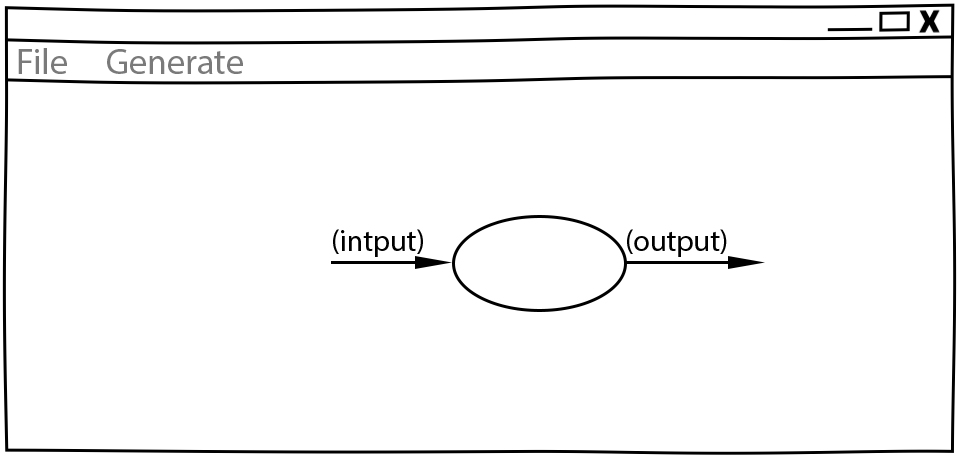
\includegraphics[width=.9\linewidth]{./img/NewCell.jpg}

\bigskip
Im folgendem einige Kerngedanken über die Funktionalität des Editors:

\begin{itemize}
\item Keine unnötigen Menuleisten, Symbolleisten, etc. Besser kontextsensitive
Kontextmenus, oder Hotkeys,  damit die Strecke, die die Maus bewegt werden muss, gering
gehalten wird.
\item Tabulatorstops einbauen, damit schnell zwischen den Textfeldern, entlang des
Graphen, gesprungen werden kann.
\item Verwendung von Drag and Drop, um eine intuitive Bedienung zum Verknüpfen von
Softwarezellen zu ermöglichen. Die Flächen, die per Drag and Drop zu Bedienen
sind, sollen über ein Maus-Hover Feedback erkennbar sein. Außerdem sollen die
Flächen nicht zu klein sein, damit ein leichtes Treffen des Feldes
sichergestellt wird. Möglicherweise können auch unsichtbare Flächen verwendet
werden, um eine Drag and Drop Fläche künstlich leicht zu vergrößern und einfacher treffbar zu machen.
\item Rectangle Selection in Kombination mit Modifier-Keys um mehrere Softwarezellen
schnell und komfortable zu selektieren.
\item Shift + Drag : Schnelles Duplizieren der selektierten Objekte. Vorbild dieser
Funktion ist 3ds Max, das dieses Bedienkonzept an vielen Stellen einsetzt.
Einmal dararn gewöhnt, möchte man es nicht mehr missen. Anwendungsfälle:
Der Anwender möchte  schnell ein gesamtes Diagramm duplizieren und an ein andere Stelle schieben, um
dort eine weitere Iteration davon zu erstellen. Möglicherweise müssen solche
Duplikate vor der Generierung des Codes aus dem Diagramm gelöscht werden.
Ein andere Anwendungsfall von Duplizierten ist, dass der Anwender eine vorhandene
Zelle an einer anderen Stelle im Diagramm verwendet möchte. Damit
entstehen weitere Probleme, bei der Generierung des Codes, das gelöst werden
muss: Duplizierte Softwarezellen müssen erkannt und nur einmal generiert werden.
\item Ctrl + Drag einer Softwarezelle: Die Softwarezelle und alle ihre Kinder werden
Verschoben. Anwendungsfall ist: Der Anwender möchte etwas Platz schaffen
zwsichen zwei Softwarezellen. Mit einem Ctrl+ Drag der zweiten Softwarezelle,
kann er diese und alle nachkommenden Softwarezellen verschieben, ohne sie
vorher extra selektieren zu müssen.
\end{itemize}

\section{Textfelder}
\label{sec:orgheadline23}
Textfelder müssen waagerecht bleiben. Auf dem Papier schreibt man die Daten auf
die Pfeile, somit wird Text auf einem schrägen Pfeil auch entlang des Striches
geschrieben.
Am Computer ist soetwas schlecht umzusetzen. Man kann Textfelder bei WPF drehen, dadurch
entsteht jedoch eine ungewohnte Bedienung beim Markiern von Text. Ein Drehen
beim Fokusieren/Defokusieren wäre auch möglich, damit wäre jedoch eine zustätzlicher
Klick nötig, falls man Text markieren möchte: Ein Mausklick zum Fokusieren/Drehen
der Textbox und ein weiterer um Text zu markieren / den Cursor zu platzieren.
Die beste Lösung wäre aus Usability-Sicht, wenn Textfelder nicht gedreht werden,
sondern immer waagerecht dargestellt werden. Somit muss hier die Notation an
manchen Stellen etwas vom orginal Abweichen.

\pagebreak
\emph{Mehrer Outputs}



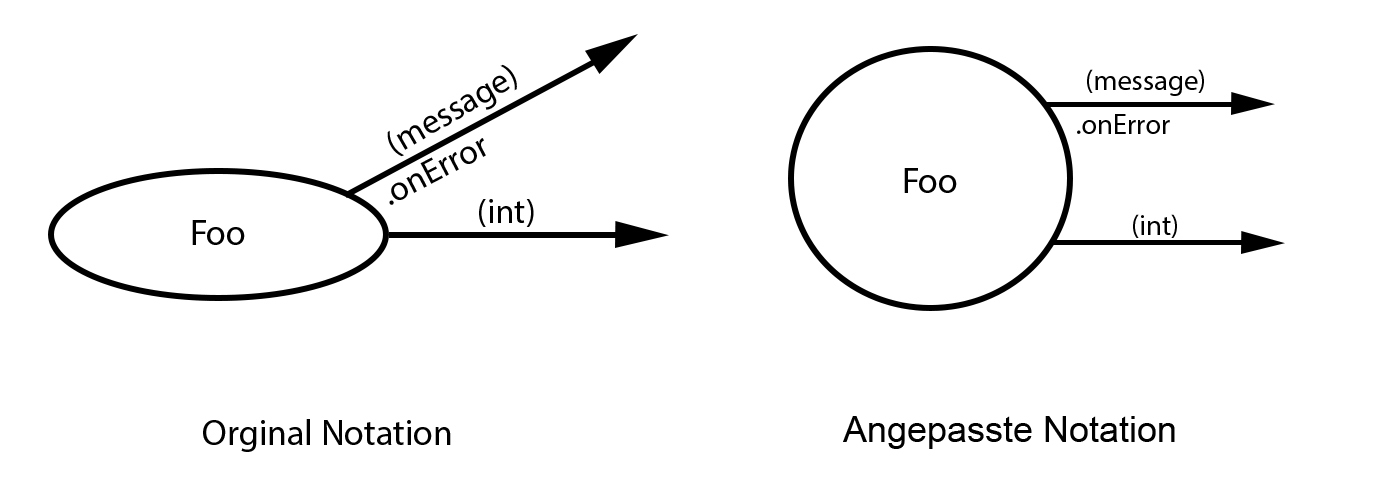
\includegraphics[width=.9\linewidth]{./img/NotationChanges1.jpg}
\bigskip

\emph{
Pfeile zwischen zwei Softwarezellen, die auf unteschiedlichen Höhen platziert
sind}

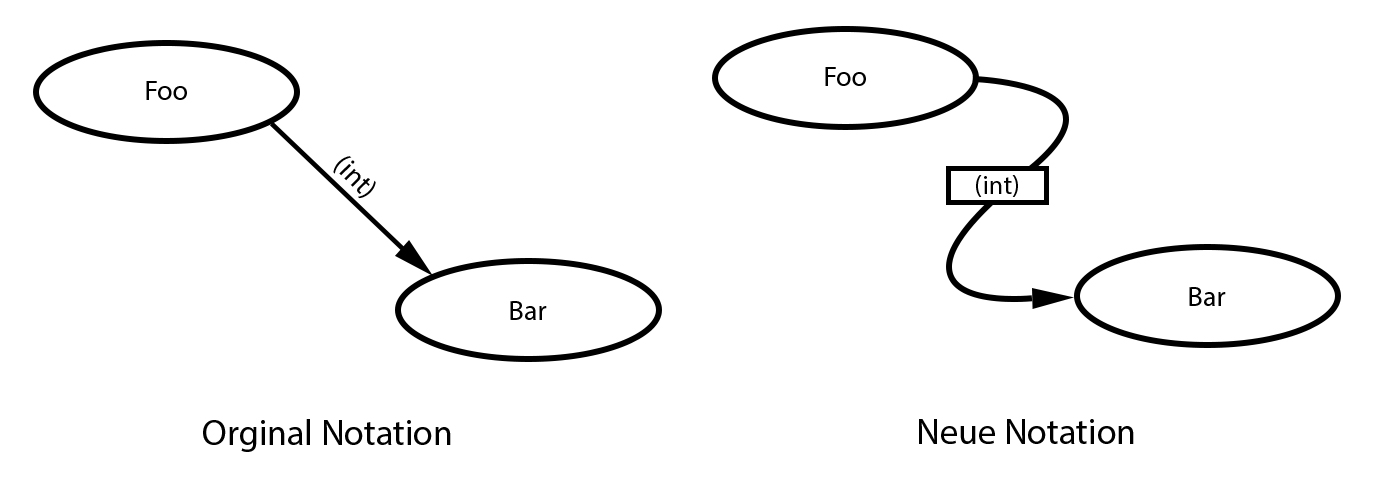
\includegraphics[width=.9\linewidth]{./img/NotationChanges2.jpg}



\section{Datentypen Organistation, Erstellung und Definition}
\label{sec:orgheadline24}
Da Flow Design auf Datenströmen arbeitet, ist das Definieren neuer Datentypen
ein wesentlicher Bestandteil davon.
Eine Möglichkeit wäre es, wie auf dem Papier, es zu erlauben an beliebigen
Stellen im Diagramm eine Box zu erstellen, in der der Anwender einen neuen
Datentyp benennen und seine Felder definieren kann. Vorteil davon wäre, dass der
Anwender die nötige Information in der Nähe des Datenstroms schnell ersichtlich
platzieren kann, wo die Daten auch vorkommen.

Nachteil wäre, dass der Algorithmus zum automatischen Spacing komplizierter
werden würde, da nun auch eine sinnvolle Platzierung der Datentypen nun mit
berücksichtigen werden müsste.
Ein weiters Problem dieser Lösung taucht auf, sobald der Anwender an unterschiedlichen
Positionen im Diagramm den selben Datentypen verwendet. In diesem Fall müssten Doppelungen erlaubt
sein, oder der Anwender würde an einer Stelle nicht die Information haben, worum
es sich bei einem Datentyp handelt.

Eine andere Option wäre es, die Datentypen nicht auf dem Drawing-Board zu
platzieren, sondern seperate vom Flow Design getrennt in einem extra UI-Element
darzustellen und dort die Defintion eigener Datentypen zu ermöglichen.
Dieses UI-Element würde in Form einer Liste alle vorhanden Datentypen
beinhalten. Zusätzliche Usability-Features wären, das Typen, die im Diagramm
vorkommen, jedoch nicht zu den Basistypen der Sprache gehören und noch nicht in
der Anwendung definiert wurden, erkannt und speziell hervorgehoben werden und
den Anwender subtil auffordert diesen zu definieren.

Um den Vorteil einer Box innerhalb des Diagrammes etwas zu entkräftigen, könnten
die Einträge in der Liste kontextsensitiv sein: Wenn der Anwender in ein
Textfeld eines Datenstromes klickt, könnte die Liste nur jene Datentypen
anzeigen, die in dem Textfeld vorhanden sind. Beim klick auf eine leere Fläche (
defokusieren des Textfeldes) würden wieder alle Datentypen im gesamten Diagramm
angezeigt werden. Desweiteren wäre eine visuelle Hervorhebung von nicht
verwendeten Datentypen auch denkbar.
\bigskip

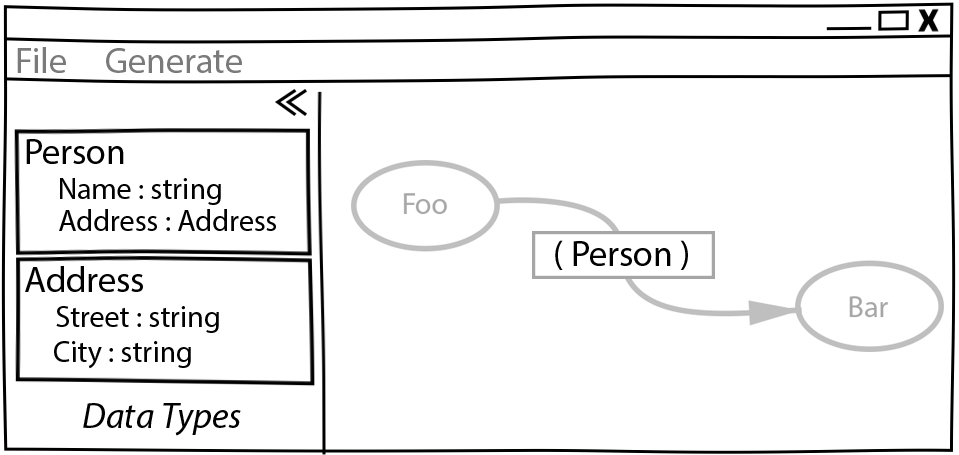
\includegraphics[width=.9\linewidth]{./img/DatatypesCrop.jpg}


Weitere Ideen wären: 
\begin{itemize}
\item Mouse-Hover über ein Datentype im Diagramm zeigt die Definition in einem Pop-Up
über dem Mauszeiger an.
\item Drag and Drop von Datentypen aus der Liste in das Drawing Board zu
ermöglichen, falls der Anwender für einen Screenshot - oder aus einem anderen
Grund - diese Information im Bild haben möchte.
\end{itemize}


\section{Realisierung/ Darstellung von Joints}
\label{sec:orgheadline25}
Datenströme können aus verschieden Quellen stammen und an einer Softwarezelle
zusammenlaufen. Flow Design bietet hierfür die Pipe-Notation, oder die s.g. Joints
an. 

\bigskip

Vorteile der Pipe-Notation / Nachteile der Joints:

\begin{itemize}
\item Einfacher zu realiseren auf GUI Seite ( Automatisches Spacing aufgrund der
wenigeren Pfeile einfacher umzusetzen
\item Pfeile müssen seltener große Distanzen überbrücken, was das Diagramm weniger
chaotisch wirken lässt
\end{itemize}

Nachteile der Pipe-Notation / Vorteile der Joints:

\begin{itemize}
\item Datenströme sind möglicherweise nicht mehr eindeutig zu interpretieren. Bei
der Verwendung von Joints ist die Herkunft eines Datenstroms eindeutig
ersichtlich. Bei der Pipe-Notation kann man diese Problem durch eine Benennung
der Datenströme lösen. Diese Erkenntnis legt eine Validierung - einschließlich
visuellem Feedback - der Datenströme auf eine eindeutige Interpretation nahe.
Eine andere Option wäre, dass man beim Generieren den Datenstrom zurückläuft
und das erste Vorkommen nimmt und nachfolgende Überschneidungen ignoriert.
\end{itemize}

Da beide Notationen ihre Vor- und Nachteile haben, soll die Anwendung beide Darstellungen unterstützen.


\section{Validierung des Datenflusses}
\label{sec:orgheadline26}
Der Validierungsprozess soll subtil sein. Ein Blockieren von Verbinden zweier
Softwarezellen soll nicht geschehen. Dies würde sonst dem Ziel entgegenstehen, 
eine möglichst freie Gestaltung, wie beim Zeichnen auf dem Papier, zu
gewährleisten. Der Anwender soll die Freiheit haben, nicht valide Verbindungen
zu erstellen, die er möglicherweise erst nach dem Verbinden dann entsprechend
anpasst. Eine dezente farbliche Hervorhebung soll als Feedback des
Validierungsprozesses ( möglicherweise indem man den Pfeil einfärbt) ausreichen. Mögliche Validierungsfehler wären:
\begin{itemize}
\item Pipe-Notation : Überschneidung von Datentypen.
\item Fehlende Daten : Nicht alle vom Input der Softwarezelle verlangten Daten
sind im Datenfluss enthalten.
\end{itemize}

Im Grunde wäre jedoch auch eine Generierung von jeglichen Flow Design Diagrammen
möglich, würde man folgende Regeln einführen:
\begin{itemize}
\item Der Graph wird zurück gelaufen, bis ein passender Datentype
gefunden wird ( Das erste Vorkommen wird genommen). Falls der Datentyp nicht
gefunden wurde, wird er in der Integration als lokale Varibale deklariert und mit einem
Default-Wert initialisiert.
\end{itemize}

\section{Validierung der Syntax}
\label{sec:orgheadline27}
Die Notation der Daten der Datenflüssen besteht aus einer einfachen Syntax. Diese muss zwingend eingehalten
 werden, damit eine Generierung des Codes möglich ist.
 Eine rote gewellte Linie unterhalb des nicht validen Textes soll dem Anwender
 anzeigen, dass ein Synatxfehler vorhanden ist.
\end{document}
